\documentclass[]{article}
\usepackage{amsmath}
\usepackage{amssymb}
\usepackage[a4paper, margin=0.8in]{geometry}
\usepackage{float}
\usepackage{caption}
\usepackage{graphicx}
\usepackage{amsthm}
\usepackage{algorithm}
\usepackage{tikz}
\usetikzlibrary{calc,positioning, arrows.meta, petri}
\usepackage{algpseudocode}
\usepackage{chngcntr}
\counterwithin{algorithm}{section}

\setlength{\parskip}{1pt}
\setlength{\parindent}{0em}


\title{Divide And Conquer}
\author{Mohammed Rizin \\ Unemployed}

\date{\today}

\theoremstyle{plain}
\newtheorem{thm}{Theorem}[section]
\theoremstyle{definition}
\newtheorem{lem}{Example}[thm]

\begin{document}
\maketitle
\begin{abstract}
    Suppose we got a bigger problem, call it $P$ of size $n$. Sometimes bigger problem are really daunting and we end up doing nothing. Instead, why don't we split the problem into multiple pieces. and solve them and combine the result. Its like we split the work into several pieces and assign to workers independently. So, each worker doesn't feel so hard about solving the problem. So we employ $DivideAndConquer$ strategy.
\end{abstract}

\section{Introduction}
\begin{center}
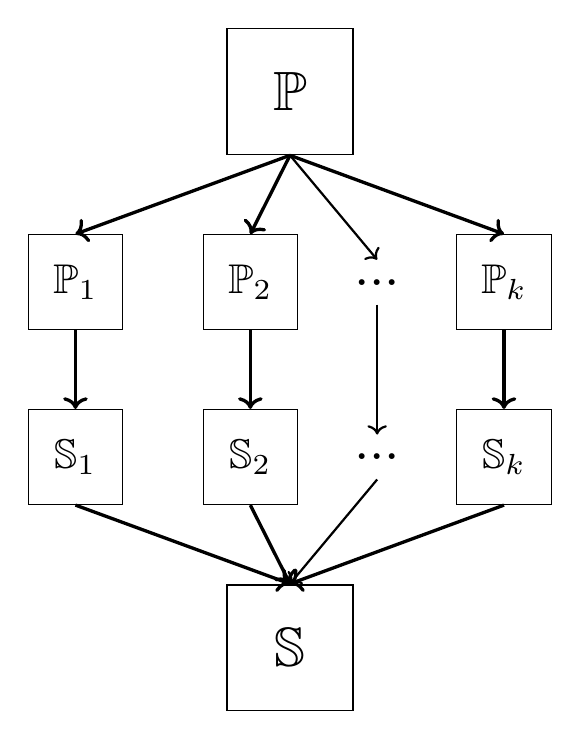
\begin{tikzpicture}[box/.style={rectangle, minimum size= 8mm, draw=black }, sibling distance = 2mm]
    \node[box, scale=2] (root) {$\mathbb{P}$};
    \node[box, scale=1.5, below left=10mm and 13mm of root] (p1) {$\mathbb{P}_1$};
    \node[box, scale=1.5, right=of p1] (p2) {$\mathbb{P}_2$};
    \node[box, scale=1.5, right=20mm of p2] (pk) {$\mathbb{P}_k$};
    \node[scale=2] (dots) at ($(p2)!0.5!(pk)$) {...};

    \node[box, scale=1.5, below=of p1] (s1) {$\mathbb{S}_1$};
    \node[box, scale=1.5, below=of p2] (s2) {$\mathbb{S}_2$};
    \node[box, scale=1.5, below=of pk] (sk) {$\mathbb{S}_k$};
    \node[scale=2] (dots2) at ($(s2)!0.5!(sk)$) {...};

    \node[box, scale=2, below right=10mm and 13mm of s1] (bigS) {$\mathbb{S}$};

    \draw[->, very thick] (root.south) -- (p1.north);
    \draw[->, very thick] (root.south) -- (p2.north);
    \draw[->, thick] (root.south) -- (dots.north);
    \draw[->, very thick] (root.south) -- (pk.north);

    \draw[->, very thick] (p1.south) -- (s1.north);
    \draw[->, very thick] (p2.south) -- (s2.north);
    \draw[->, very thick] (pk.south) -- (sk.north);
    \draw[->, thick] (dots.south) -- (dots2.north);

    \draw[->, very thick] (s1.south) -- (bigS.north);
    \draw[->, very thick] (s2.south) -- (bigS.north);
    \draw[->, thick] (dots2.south) -- (bigS.north);
    \draw[->, very thick] (sk.south) -- (bigS.north);

\end{tikzpicture}
\end{center}

As discussed earlier, we are dividing a task into several pieces and solve them individually and independently. 

\subsection{Conditions for Divide and Conquer}
\begin{enumerate}
    \item All the sub-problems should be the same task as the main problem.
    \item There should be an known method to combine the solutions at least
\end{enumerate}

Since all the sub-problems are the same task as the parent problem, This is a recursive algorithm. 

\subsection{Applications of Divide and Conquer}
\begin{enumerate}
    \item Binary search
    \item Finding Minimum and Maximum
    \item Merge Sort
    \item Quick Sort
    \item Stressen's Matrix Multiplication
\end{enumerate}

\section{Recurrence Relation}
To analyze the time complexity of divide and conquer algorithms, we often use recurrence relations. For example:

\begin{verbatim}
void Test(int n){
    if (n > 0){
        printf("%d", n);
        Test(n-1);
    }
}

Test(3)
\end{verbatim}


\begin{center}
    \begin{tikzpicture}[box/.style={rectangle, minimum size=8mm, draw=black}, 
        sibling distance=2.5cm, 
        level distance=2cm,
        % edge from parent path={(\tikzparentnode.south) -- (\tikzchildnode.north)}
    ]
        \node {Test(3)}
        child { node {3} }
        child { node {Test(2)}
            child { node {2} }
            child { node {Test(1)}
                child { node {1} }
                child { node {Test(0)}
                    child{node {$\mathsf{X}$}
                } 
            }
        }
    };
    \end{tikzpicture}
\end{center}

Since the only statement in the function is printf, which take $O(1)$ time, at each recursive step $O(1)$ is done. If $Test(n)$ is executed, the number of recursive calls are $n+1$, the number of printf calls are $n$.
So the time complexity of this algorithm is $On(n)$

This won't be possible in every algorithm to open the function and count them and make assumption about $n$ cases. Mathematically, That is not sufficient. Thus, Recurrence Relation Come into play.

Lets take the same code we used before:

\begin{algorithm}[H]
    \caption{Simple Printing with recursion}
    \label{printRecursion}
    \begin{algorithmic}
        \Procedure{Test}{int $n$} \Comment{Assume it takes $T(n)$}
        \If{$n > 0$} 
            \State$print(n)$ \Comment{$O(1)$}
            \State$Test(n-1)$  \Comment{$T(n-1)$}
        \EndIf
        \EndProcedure
    \end{algorithmic}
\end{algorithm}

So,

\[
\begin{aligned}
    T(n) &=
    \begin{cases}
        T(n - 1) + 1 \label{base} & n > 0, \\
        1 & n = 0
    \end{cases} \\
    \because \hspace{10pt} T(n) &= T(n - 1) + 1, \\
    T(n - 1) &= T(n - 2) + 1, \\
    \text{Substituting} & \text{(3) in (1)}, \\
    T(n) &= [T(n - 2) + 1] + 1 = T(n - 2) + 2, \\
    T(n) &= [T(n - 3) + 1] + 2 = T(n - 3) + 3, \\
    T(n) &= \hspace{7pt}\vdots \hspace{7pt}+\hspace{7pt} \vdots, \\
    T(n) &= T(n - k) + k, \\
    \because \hspace{10pt} T(0) &= 1, \\
    \text{if (k = n)}, \\
    T(n) &= T(0) + n, \\
    T(n) &= 1 + n.\\
    \text{This algorithm is } & O(n)
\end{aligned}
\]

Lets look Another example
\begin{algorithm}[H]
    \caption{Recursion with simple For Loop}
    \label{printRecursion}
    \begin{algorithmic}
        \Procedure{Test}{int $n$} \Comment{Assume it takes $T(n)$}
        \If{$n > 0$} 
            \For{$i \gets 0$ to $n-1$} \Comment{$n-1$}
                \State$print(n)$ \Comment{Everything inside for will be $T(n) = n$}
            \EndFor
            \State$Test(n-1)$  \Comment{$T(n-1)$}
        \EndIf
        \EndProcedure
    \end{algorithmic}
\end{algorithm}

So,

\[
\begin{aligned}
    T(n) &= T(n - 1) + 2n + 2\\
    \text{We need to take Asymptotic Notation}\\
    T(n) &\simeq  T(n - 1) + n\\
    T(n) &=
    \begin{cases}
        T(n - 1) + n \label{base} & n > 0, \\
        1 & n = 0
    \end{cases} \\
    \because \hspace{10pt} T(n) &= T(n - 1) + n, \\
    T(n - 1) &= T(n - 2) + n - 1, \\
    \text{Substituting} & \text{(3) in (1)}, \\
    T(n) &= [T(n - 2) + n - 1] + n = T(n - 2) + (n-1) + n, \\
    T(n) &= [T(n - 3) + n - 2] + (n-1) + n = T(n - 3) + (n-2) + (n-1) + n, \\
    T(n) &= \hspace{7pt}\vdots \hspace{7pt}+\hspace{7pt} \vdots, \\
    T(n) &= T(n - k) + (n-(k - 1 )) + \cdots + (n-1) + n, \\
    \because \hspace{10pt} T(0) &= 1, \\
    \text{if (k = n)}, \\
    T(n) &= T(0) + \frac{n(n+1)}{2} = 1 + \frac{n(n+1)}{2}, \\
    T(n) &\approx \frac{n(n+1)}{2}  \approx \frac{n^2+n}{2}\\
    \text{This algorithm is } & O(n^2)
\end{aligned}
\]

Lets look Another example
\begin{algorithm}[H]
    \caption{Recursion with for loop \textbf{Step = $2 \cdot i$} }
    \label{printRecursion}
    \begin{algorithmic}
        \Procedure{Test}{int $n$} \Comment{Assume it takes $T(n)$}
        \If{$n > 0$} 
            \For{$i \gets 0$ \textbf{to} $n-1$ \textbf{step} $2 \cdot i$} \Comment{This is $\log(n) + 1$ Not useful. }
                \State$print(n)$ \Comment{This takes $ \log{n}$}
            \EndFor
            \State$Test(n-1)$  \Comment{$T(n-1)$} 
        \EndIf
        \EndProcedure
    \end{algorithmic}
\end{algorithm}

Although I know we excluded many of the time complexities simply because we wont using it in asymptotic equation

\begin{align*}
    \text{After taking Asymptotic Notation}\\
    T(n) &= T(n - 1) + \log{n} \tag{1} \label{base}\\
    T(n) &=
    \begin{cases}
        T(n - 1) + \log{n} & n > 0, \\
        1 & n = 0
    \end{cases} \tag{2} \\  
    \because \hspace{10pt} T(n) &= T(n - 1) + \log{n}  \\
    T(n - 1) &= T(n - 2) + \log{(n - 1)} \tag{3} \label{downStep}\\
    \text{Substituting eqn } (\ref{downStep}) \text{ in } (\ref{base}),  \\
    T(n)&= [T(n - 2) + \log(n - 1)] + \log(n)\\ 
        &= T(n - 2) + \log(n-1) + \log{n}\\ &= T(n-2) + \log (n^2-n), \\
    T(n)&= [T(n - 3) + n - 2] + (n-1) + n \\
        &= T(n - 3) + \log(n-2) + \log(n-1) + \log n\\
        &= T(n-3) + \log ((n-2) \cdot (n-1) \cdot(n)) \\
    T(n) &= T(n-k) + \log{\left(\prod_{i=0}^{k-1} (n-i) \right)} \label{kSteps} \tag{4}\\
    T(n) &= T(n-k) + \log \left(\frac{n!}{n-(k-2)!}\right)\\
    \because \hspace{10pt} T(0) &= 1, \\
    \text{if (k = n)}, \\
    T(n) &= T(0) + \log \left( \frac{n!}{2}\right) = 1 + \cdot \left( \frac{n!}{2}\right) \\
    T(n) &\approx \log{n!}  \approx \log{n!}\\
    \text{Upper bound of }& \log{n!}  \text{ is }O(n \cdot \log{n})\\
    \text{This algorithm is } & O(n \cdot \log{n})\\
    OR & \\
    \text{From eqn (\ref{kSteps})}:\\
    T(n) &= T(n-k) + \log{\left(\prod_{i=0}^{k-1} (n-i) \right)}\\
    \text{By Binomial Theorem, }\\
    T(n) &= T(n-k) + \log{(n^k + \cdots) }\\
    T(n) &\approx T(n-k) + k \cdot \log {n}\\
    \because \hspace{10pt} T(0) &= 1, \\
    \text{if (k = n)}, \\
    T(n) &= T(0) + n \cdot log{n}\\
    \text{This algorithm is } & O(n \cdot \log{n})
\end{align*}

    By observing above examples, we can observe that for any decreasing recurrence relation function i.e. ($T(n) = T\underbrace{(n-1)}_{Decreasing} + anything$) is O($n \cdot anything$)

$T(n) = T(n-2) + 1 = 1 + \frac{n}{2} \longrightarrow O(n) $

$T(n) = T(n-100) + n = 1 + \frac{n(n+1)}{200} \longrightarrow O(n^2) $
\\\\
\textbf{But what if $T(n) = 2 \cdot T(n -1) + 1$ :}
\begin{algorithm}[H]
    \caption{Multiple Recursion}
    \label{printRecursion}
    \begin{algorithmic}
        \Procedure{Test}{int $n$} \Comment{Assume it takes $T(n)$}
        \If{$n > 0$} 
            \State$print(n)$ \Comment{$O(1)$}
            \State$Test(n-1)$  \Comment{$T(n-1)$}
            \State$Test(n-1)$  \Comment{$T(n-1)$}
        \EndIf
        \EndProcedure
    \end{algorithmic}
\end{algorithm}

\begin{center}
    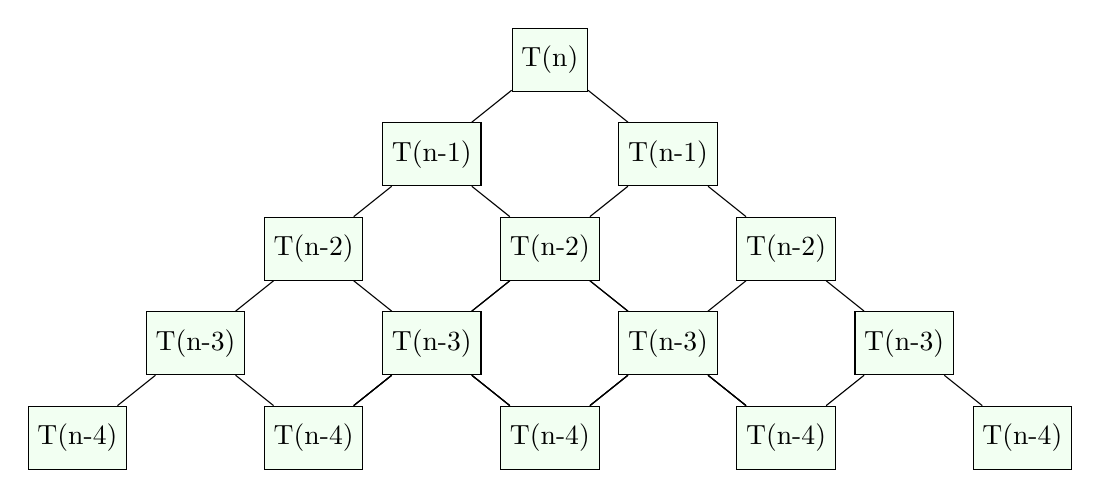
\begin{tikzpicture}[
        box/.style={rectangle, draw=green!60, fill=green!5, minimum size=8mm, draw=black}, 
        level distance=1.2cm, % Adjusted for balance
        sibling distance=3cm % Prevents overlap
    ]
        \node[box] {T(n)}
            child { node[box] {T(n-1)}
                child { node[box] {T(n-2)}
                    child { node[box] {T(n-3)}
                        child { node[box] {T(n-4)} }
                        child { node[box] {T(n-4)} }
                    }
                    child { node[box] {T(n-3)}
                        child { node[box] {T(n-4)} }
                        child { node[box] {T(n-4)} }
                    }
                }
                child { node[box] {T(n-2)}
                    child { node[box] {T(n-3)}
                        child { node[box] {T(n-4)} }
                        child { node[box] {T(n-4)} }
                    }
                    child { node[box] {T(n-3)}
                        child { node[box] {T(n-4)} }
                        child { node[box] {T(n-4)} }
                    }
                }
            }
            child { node[box] {T(n-1)}
                child { node[box] {T(n-2)}
                    child { node[box] {T(n-3)}
                        child { node[box] {T(n-4)} }
                        child { node[box] {T(n-4)} }
                    }
                    child { node[box] {T(n-3)}
                        child { node[box] {T(n-4)} }
                        child { node[box] {T(n-4)} }
                    }
                }
                child { node[box] {T(n-2)}
                    child { node[box] {T(n-3)}
                        child { node[box] {T(n-4)} }
                        child { node[box] {T(n-4)} }
                    }
                    child { node[box] {T(n-3)}
                        child { node[box] {T(n-4)} }
                        child { node[box] {T(n-4)} }
                    }
                }
            };
    \end{tikzpicture}
\end{center}

The algorithm time depends on the number of level. At a certain level k the time taken is $2^k$. Then 
$T(n) = 2^0 + 2^1 + 2^2 + \cdots + 2^k = 2^{k+1} - 1 $

Assume $n = k$,
Then it is $2^{n+1} - 1$. That is $O(2^n)$.
\[
\begin{aligned}
    T(n) &=
    \begin{cases}
        2\cdot T(n - 1) + 1 \label{base} & n > 0, \\
        1 & n = 0
    \end{cases} \\
    \because \hspace{10pt} T(n) &= T(n - 1) + 1, \\
    T(n - 1) &= 2\cdot T(n - 2) + 1, \\
    \text{Substituting} & \text{(3) in (1)}, \\
    T(n) &= 2\cdot[2 \cdot T(n - 2) + 1] + 1 = 4 \cdot T(n - 2) + 3, \\
    T(n) &= 4\cdot[2 \cdot T(n - 3) + 1] + 3 = 8 \cdot T(n - 3) + 7, \\
    T(n) &= \hspace{7pt}\vdots \hspace{7pt}+\hspace{7pt} \vdots, \\
    T(n) &= 2^k \cdot T(n - k) + 2^k - 1, \\
    \because \hspace{10pt} T(0) &= 1, \\
    \text{if (k = n)}, \\
    T(n) &= 2^n \cdot T(0) + 2^n - 1, \\
    T(n) &= 2^{n+1} - 1.\\
    \text{This algorithm is } & O(2^n)
\end{aligned}
\]

\section{Master Theorem for Decreasing}
\begin{thm}
    If $T(n) = a \cdot T(n-1) + f(n)$ where $a > 0$, $b > 0$, and $f(n) = O(n^k)$ where $k \geq 0$, then:
    \[
    \begin{cases}
        O(n^{k}) \text{ or } O(f(n)) & \text{if } 0 < a < 1, \\
        O(n^{k+1}) \text{ or } O(n \cdot f(n)) & \text{if } a = 1, \\
        O(n^{k} \cdot a^{\frac{n}{b}}) \text{ or } O(a^{\frac{n}{b}} \cdot f(n)) & \text{if } a > 1.
    \end{cases}
    \]
\end{thm}

\begin{lem}
$T(n) = T(n - 1) + 1 \rightarrow O(n)$
\end{lem}

\begin{lem}
    $T(n) = T(n - 1) + n \rightarrow O(n^2)$
\end{lem}

\begin{lem}
    $T(n) = T(n - 1) + \log{n} \rightarrow O(n\cdot \log{n})$
\end{lem}

\begin{lem}
    $T(n) = 2\cdot T(n - 1) + 1 \rightarrow O(2^n)$
\end{lem}

\begin{lem}
    $T(n) = 2\cdot T(n - 1) + 1 \rightarrow O(3^n)$
\end{lem}
\begin{lem}
    $T(n) = 3\cdot T(n - 1) + n \rightarrow O(n\cdot 3^n)$
\end{lem}

\section{Recurrence Relation in Dividing Function.}
So far we have seen decreasing function and master theorem for decreasing function as well. But what if the value is down by a ratio inside the same function. 

If the ratio $r$ is greater than or equal to 1 then This function would go infinity (i.e. we multiply it with positive ratio, and the value never stops). So we use a ratio that $0 < r < 1$, i.e. we divide by some value.

Lets see some examples:
\begin{lem}
\textbf{$T(n) = 2 \cdot T(n -1) + 1$ :}
\begin{algorithm}[H]
    \caption{Recursion with Division}
    \label{SimpleDivisionRecursion}
    \begin{algorithmic}
        \Procedure{Test}{int $n$} \Comment{$T(n)$}
        \If{$n > 0$} 
            \For{$i \gets 0$ \textbf{to} $n-1$} 
            \State$print(n)$ \Comment{$O(n)$}
            \EndFor
            \State$Test(n/2)$  \Comment{$T(n/2)$}
            \State$Test(n/2)$  \Comment{$T(n/2)$}
        \EndIf 
        \EndProcedure
        \Comment {$T(n) = T(\frac{n}{2}) + 1$}
    \end{algorithmic}
\end{algorithm}
\end{lem}

Let us draw the tree:
In this tree we are only including the time taken for the purpose of viewing it

\begin{center}
    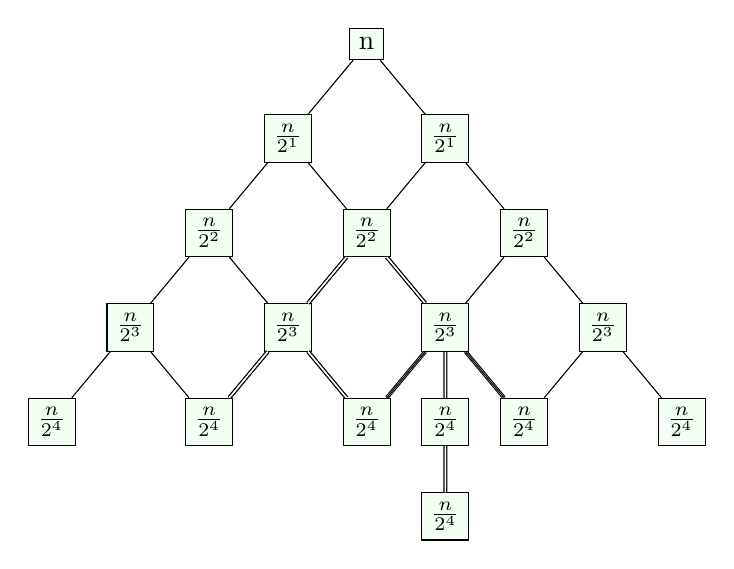
\begin{tikzpicture}[
        box/.style={rectangle, draw=green!60, fill=green!5, minimum size=4mm, draw=black}, 
        level distance=1.2cm, % Adjusted for balance
        sibling distance=2cm % Prevents overlap
    ]
        \node[box] {n}
            child { node[box] {$\frac{n}{2^1}$}
                child { node[box] {$\frac{n}{2^2}$}
                    child { node[box] {$\frac{n}{2^3}$}
                        child { node[box] {$\frac{n}{2^4}$} }
                        child { node[box] {$\frac{n}{2^4}$} }
                    }
                    child { node[box] {$\frac{n}{2^3}$}
                        child { node[box] {$\frac{n}{2^4}$} }
                        child { node[box] {$\frac{n}{2^4}$} }
                    }
                }
                child { node[box] {$\frac{n}{2^2}$}
                    child { node[box] {$\frac{n}{2^3}$}
                        edge from parent [double]
                        child { node[box] {$\frac{n}{2^4}$} 
                        edge from parent [double]}
                        child { node[box] {$\frac{n}{2^4}$} 
                        edge from parent [double]}
                    }
                    child { node[box] {$\frac{n}{2^3}$}
                        edge from parent [double]
                        child { node[box] {$\frac{n}{2^4}$} edge from parent [double]
                        child { node[box] {$\frac{n}{2^4}$} 
                        edge from parent [double]}
                    }
                }
                }}
            child { node[box] {$\frac{n}{2^1}$}
                child { node[box] {$\frac{n}{2^2}$}
                    child { node[box] {$\frac{n}{2^3}$}
                        edge from parent [double]
                        child { node[box] {$\frac{n}{2^4}$} 
                        edge from parent [double]}
                        child { node[box] {$\frac{n}{2^4}$} 
                        edge from parent [double]}
                    }
                    child { node[box] {$\frac{n}{2^3}$}
                        edge from parent [double]
                        child { node[box] {$\frac{n}{2^4}$} 
                        edge from parent [double]}
                        child { node[box] {$\frac{n}{2^4}$} 
                        edge from parent [double]}
                    }
                }
                child { node[box] {$\frac{n}{2^2}$}
                    child { node[box] {$\frac{n}{2^3}$}
                        child { node[box] {$\frac{n}{2^4}$} }
                        child { node[box] {$\frac{n}{2^4}$} }
                    }
                    child { node[box] {$\frac{n}{2^3}$}
                        child { node[box] {$\frac{n}{2^4}$} }
                        child { node[box] {$\frac{n}{2^4}$} }
                    }
                }
            };
    \end{tikzpicture}
\end{center}

If we add the time in each level:\\ 
\begin{flalign*}
\text{Level 1 : }&n \\
\text{Level 2 : }&\frac{n}{2} + \frac{n}{2} = n \\
\text{Level 3 : }&\frac{n}{4} + \frac{n}{4} + \frac{n}{4} + \frac{n}{4} = n \\
\text{Level 4 : }&\frac{n}{8} + \frac{n}{8} + \frac{n}{8} + \frac{n}{8} + \frac{n}{8} + \frac{n}{8} + \frac{n}{8} + \frac{n}{8} = n\\
\end{flalign*}



\begin{proof}[Lets Solve it!]
    As we go down we find that at each level it takes $n$ time.
    The Time Function of this algorithm is :
    \begin{equation}\label{timeFunc}
        T(n) =  
        \begin{cases}
            1 & n = 1\\
            2T(n/2) + n & n > 1 \\
        \end{cases}
    \end{equation}
    The equation (\ref{timeFunc}) after k step would have $\frac{n}{2^k}$, and there would be k leafs in the tree.
    As this tree goes on and on. Finally, it will terminate after T(1). 
    Assume $T(\frac{n}{2^k}) = T(1)$
    \begin{align*}
        \frac{n}{2^k} &= 1\\
        n &= 2^k\\
        k &= \log_2{n}
    \end{align*}
    So, the total height of the tree is $\log{n}$ and the time taken in each level is n. \\
    So the total time $T(n) = n\cdot \log{n}$\\
    So this algorithm have $O(n\cdot \log{n})$
\end{proof}

Let's Solve it by Recurrence Relation: 

When we look at equation \ref{timeFunc}, 
\begin{align*}
    T(n) &= 2\cdot T\left(\frac{n}{2}\right) + n \tag{1} \label{base}\\ 
    T\left(\frac{n}{2}\right) &= 2\cdot T\left(\frac{n}{2} \cdot \frac{n}{2}\right) + \frac{n}{2} = 2\cdot T\left(\frac{n}{2^2}\right) + \frac{n}{2} \tag{2} \label{halfTime}
    \\
    \text {Substituting equation } &\text{(\ref{halfTime}) in (\ref{base})}\\
    T(n) &= 2\cdot [2\cdot T\left(\frac{n}{2^2}\right) + \frac{n}{2} ] + n\\
    T(n) &= 2^2\cdot T\left(\frac{n}{2^2}\right) + n  + n \tag{3} \label{eqn2}\\
    \text{Further if we find } &T\left(\frac{n}{2^2}\right)\\
    T(n) &= 2^3\cdot T\left(\frac{n}{2^3}\right) + 3n \tag{3} \label{eqn2}\\
    T(n) &= \vdots  + \vdots \text { After k steps} \\ 
    T(n) &= 2^k \cdot T\left(\frac{n}{2^k}\right) + kn \tag{4} \label{eqnk}\\
    \text{Assume } \frac{n}{2^k} &= 1\\
    n &= 2^k \tag{5} \label{n_value}\\ 
    k &= \log_2{n} \tag{6} \label{k_value} \\
    \text{Subtituting  (\ref{k_value})}& \text{(\ref{n_value}) in equation (\ref{eqnk})}\\
    T(n) &= n \cdot T(1) + n\cdot \log{n}\\
    T(n) &= n + n\cdot \log{n}\\
    \text{So the algorithm has } &\text{a time complexity of } O(n\log n)
\end{align*}

\section{Master's Theorem for Dividing Functions}




\end{document} 
